% %
% LAYOUT_E.TEX - Short description of REFMAN.CLS
%                                       99-03-20
%
%  Updated for REFMAN.CLS (LaTeX2e)
%
\documentclass[twoside,a4paper]{refart}
\usepackage{makeidx}
\usepackage{float}
\usepackage{ifthen}
\usepackage{graphicx}
% ifthen wird vom Bild von N.Beebe gebraucht!

\def\bs{\char'134 } % backslash in \tt font.
\newcommand{\ie}{i.\,e.,}
\newcommand{\eg}{e.\,g..}
\DeclareRobustCommand\cs[1]{\texttt{\char`\\#1}}

\title{A Guide on Modelling Synapses in CellBlender and MCell}
\author{Jaron Lee}

\date{}
\emergencystretch1em  %

\makeindex 

\setcounter{tocdepth}{2}

\begin{document}

\maketitle

\begin{abstract}
\end{abstract}

%\marginlabel{Start Blender}
\newpage


%%%%%%%%%%%%%%%%%%%%%%%%%%%%%%%%%%%%%%%%%%%%%%%%%%%%%%%%%%%%%%%%%%%%

\section{Pre- and Postsynaptic Genomtry with Blender}
This section follows the paper written by Czech et. al. closely.

\subsection{Creating a Spine Head}

\begin{enumerate}

\item   Open Blender. In the '3D View' pane, delete the default object (shortcut: x)
    
\item   Create a sphere. Select the 'UV Sphere' option from the sidebar. Below a pane called 'Add Circle' appears; set 'Segments' and 'Rings' to 16, 'Radius to '0.25'. 
        \begin{figure}[H]
        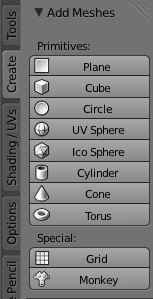
\includegraphics[scale=0.5]{spinehead1.png}
        \end{figure}

\item   Rename the sphere. Double-click the entry box below to change the default name to 'SpineHead'.
        \begin{figure}[H]
        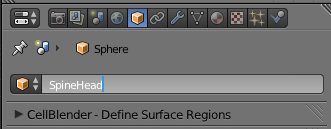
\includegraphics[scale=0.5]{spinehead2.png}
        \end{figure}

\item   Change view to see the sphere from the 'Front' view. (shortcut: 1 on numpad)

\item   Deselect the sphere (shortcut: a) and make it transparent (shortcut: z)

\item   Select the vertices to be removed. First, switch from 'Object Mode' to 'Edit Mode'. Ensure that 'Edge select' is enabled. Then use box select (shortcut: b) to capture only the faces that make up the top half of the sphere. Delete these faces (shortcut: x) and select the 'Faces' option in the delete menu.
        \begin{figure}[H]
        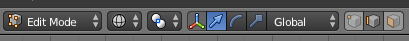
\includegraphics[scale=0.5]{spinehead3.png}
        \end{figure}

\item   Close the opening. Select the topmost vertices (remaining in 'Edge select' mode) using box select (shortcut: b). Then, extrude (shortcut: e) and click 'Edges Only' under 'Extrude' in 'Mesh Tools'.        
        \begin{figure}[H]
        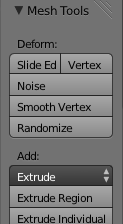
\includegraphics[scale=0.5]{spinehead4.png}
        \end{figure}
        Set the extrude distance by pressing 0 and Enter to confirm. Scale the extrusion by pressing s, 0 and Enter to confirm. Select 'Remove Doubles' under 'Mesh Tools' to remove the duplicated vertices and reconnect the triangles. Blender should note that you remove 15 vertices as a result.
        \begin{figure}[H]
        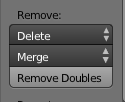
\includegraphics[scale=0.5]{spinehead5.png}
        \end{figure}
        The object should now be closed by a flat top.

\item   Subdivide triangles at the top. Unfortunately the 'Multicut tool' has been deprecated. To create set of concentric rings, first select the topmost vertices (shortcut: b). Then enter 'Knife' mode (shortcut: k), and hold down \textit{control}. This locks the knife cut to the midpoint. Click around to make a circle cut, and then press \textit{Enter} to complete the cut. Continue these cuts until the picture looks as below:
        \begin{figure}[H]
        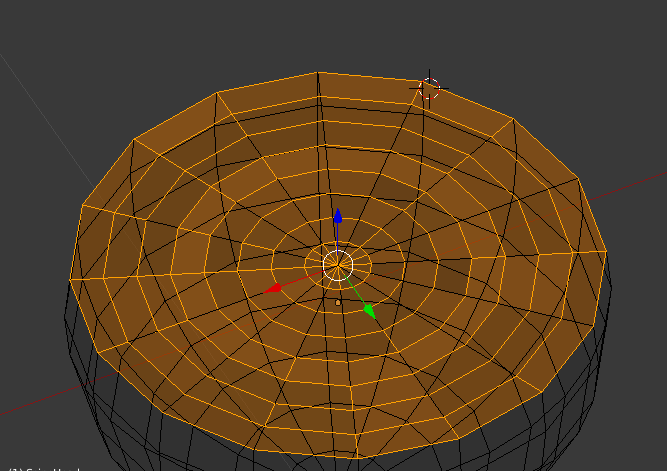
\includegraphics[scale=0.5]{spinehead6.png}
        \end{figure}
         
\end{enumerate}

\subsection{Creating a presynaptic bouton}

\begin{enumerate}
    \item   Duplicate the \textit{spine.blend} file as \textit{bouton.blend}. in \textit{bouton.blend} deselect all (shortcut: a).
    
\item   Duplicate the spine head and rotate. First, switch to 'Front' view (shortcut: 1 on numpad). Duplicate (shortcut: Shift-d, Enter) and rotate 180 degrees (shortcut: r, 180, Enter). To separate the selection of the spine heads, press p and click 'Selection'.

\item   Rename the item. Switch to 'Object Mode' (shortcut: Tab) and edit the name field to 'PresynapticBouton'.
        \begin{figure}[H]
        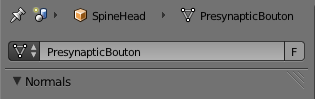
\includegraphics[scale=0.5]{bouton1.png}
        \end{figure}

\item   Shift and scale the bouton. Grab the object (shortcut: g), constrain movement to the z-axis (shortcut: z) and type 0.15, \textit{Enter} to move the object. Scale the object to be 20\% larger by typing s, 1.2, \textit{Enter}.

\item   Creating the invagination. Switch to 'Edit Mode' (shortcut: Tab) and deselect everything (shortcut: a). Select the lowermost vertices (see below) and perform the 'Select Less' operation (shortcut: Control-Minus on numpad). Click the 'Extrude Region' button under 'Add' in 'Tools', press z to constrain, and type -0.075 to extrude it upwards.
        \begin{figure}[H]
        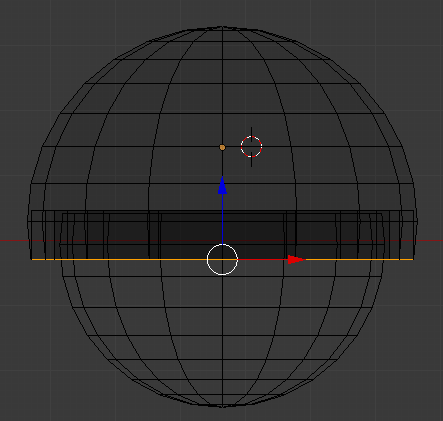
\includegraphics[scale=0.5]{bouton2.png}
        \end{figure}

\end{enumerate}

\end{document}
